\section[Intro]{Introduction}

% Add outline page for Introduction section
\begin{frame}{Outline}
    \tableofcontents[currentsection, sectionstyle=show/hide, subsectionstyle=show/show/hide, subsubsectionstyle=hide/hide/hide]
\end{frame}


\subsection{Information Theory}
\begin{frame}[fragile]{Information Theory\refer{1}}
    \begin{itemize}
        \item 1948 Claude Shannon: "A Mathematical Theory of Communication" 
        \item Self-information \\ a symbol of probability $\mathit{p}$ contains $\mathit{log}_2{1\over \mathit{p}}$ bits of information.
        \item Shannon Entropy \\Let $\mathit{X}$ be a random variable, which takes values in the set $\mathcal{X}$ and is distributed according to $\mathit{p}$ \\ $$\mathit{H(X) = \sum_{x \in \mathcal{X}} p(x)} \mathit{log}_2 {1\over{\mathit{p(x)}}}$$ 
    \end{itemize}
\end{frame}

\subsection{Source Coding Theorem}
\begin{frame}[fragile]{Source Coding Theorem (Shannon) \refer{1}}
    \begin{itemize}
        \item prerequisite: lossless data compression
        \item $\mathit{H(X)}$ is compression limit, i.e. lower bound $\mathit{L_{\text{avg}} \geq H(X)}$ \\ 
        which measures \textbf{the minimum average number of bits} needed to encode \textbf{a symbol} from a data source
        \item $\mathit{H(X)}$ is achievable, $\mathit{L_{\text{avg}} \rightarrow H(X)}$ \\
        for a sufficiently long sequence of symbols it is possible to achieve an average code length close to $\mathit{H(X)}$
        \item Shannon's Source Coding Theorem \refer{1} $$\mathit{N \cdot H(X)}$$
    \end{itemize}
\end{frame}

\subsection{Entropy Coding}
\begin{frame}[fragile]{Entropy Coding}
    \begin{itemize}
        \item Implementation of Shannon's Source Coding Theorem
        \item High-probability symbols get shorter codes
        \item Low-probability symbols get longer codes.
        \item A method that attempts to approach the lower bound $\mathit{H(X)}$
        \item Entropy Coding Family
        \begin{itemize}
            \item Huffman Coding: ZIP, JPEG, PNG
            \item Arithmetic Coding/Range Coding: JPEG, H.264, HEVC.
            \item Asymmetric Numeral System (ANS): Zstandard, JPEG XL, AVIF
        \end{itemize}
    \end{itemize}
\end{frame}
\begin{frame}[fragile]{Huffman Coding}
    \begin{center}
        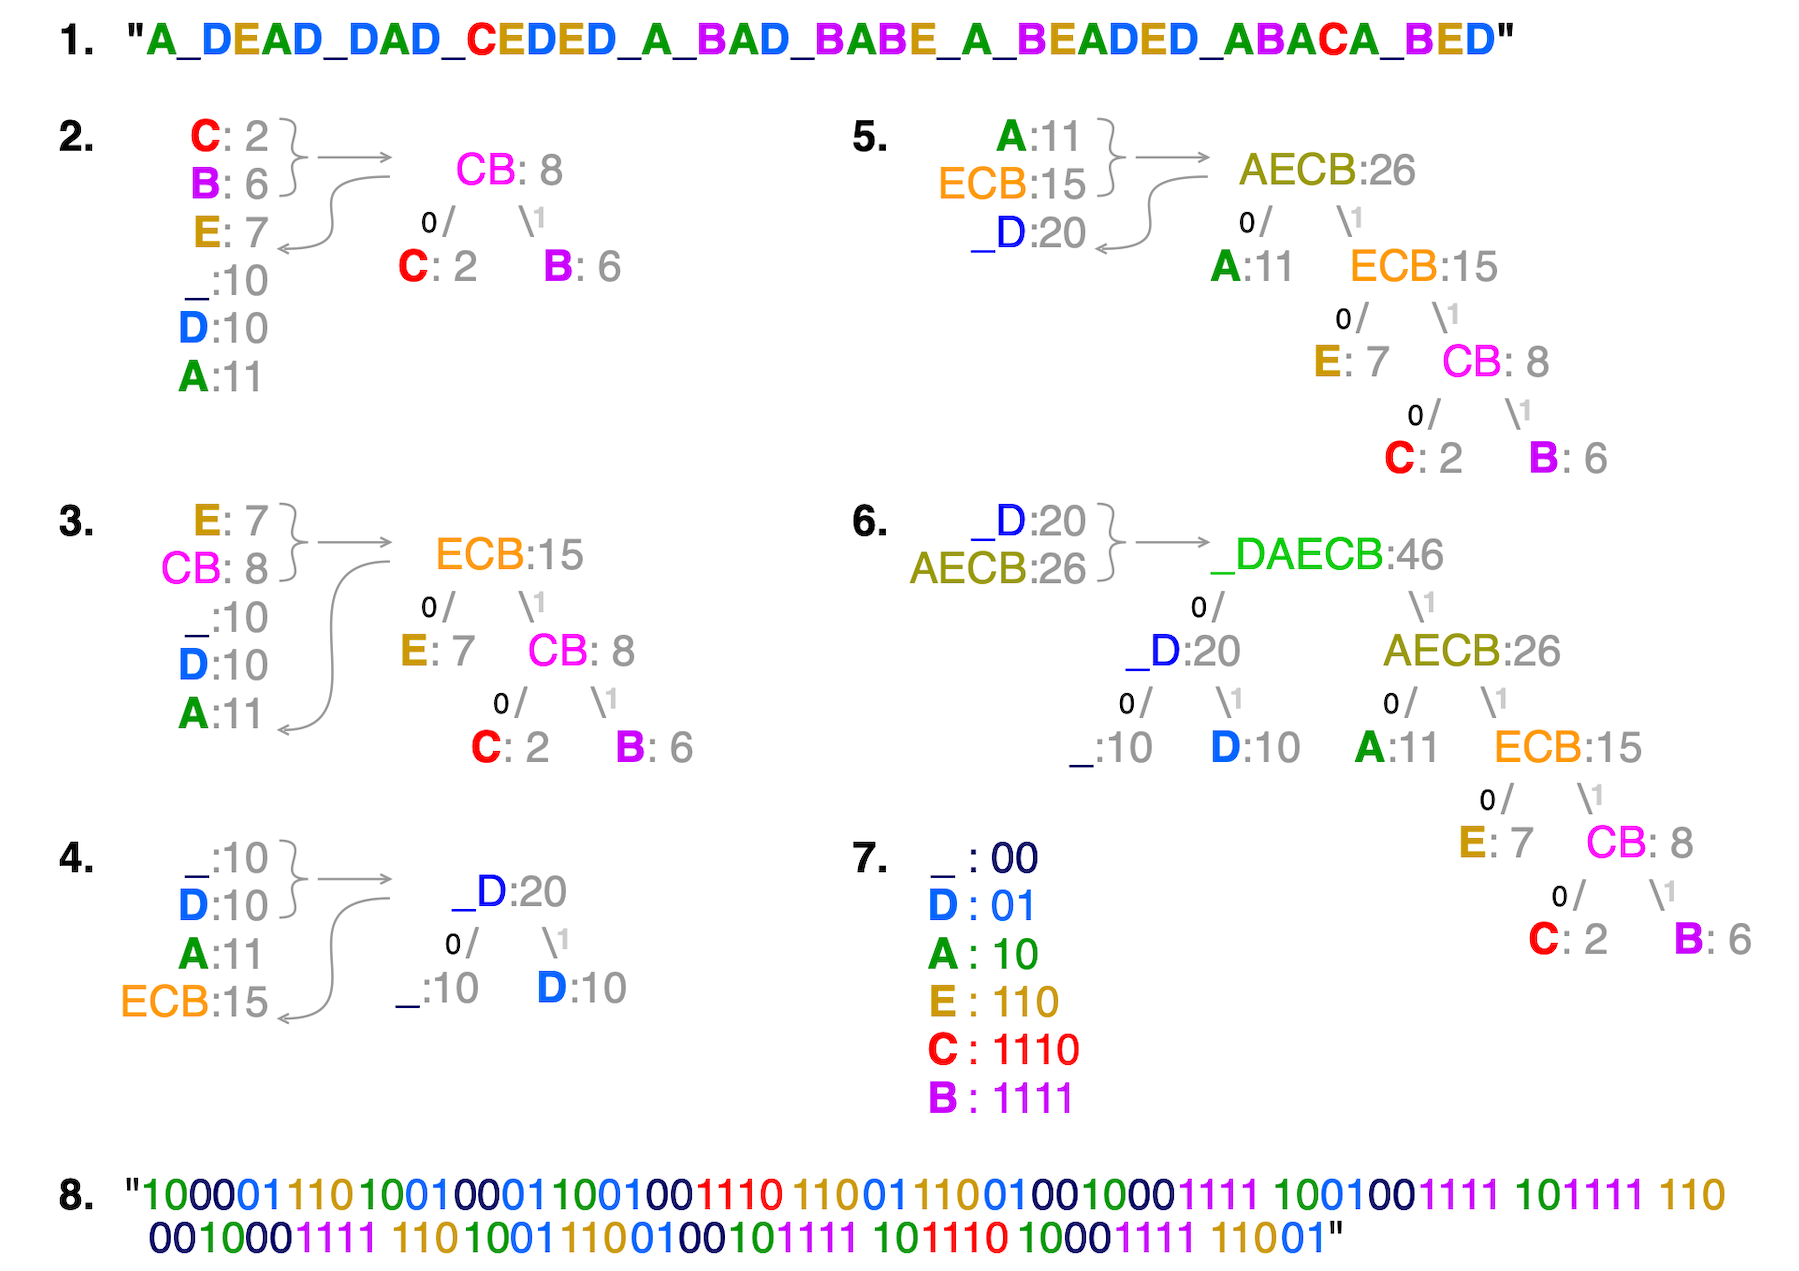
\includegraphics[width=0.6\textwidth]{../24ws_ANS.assets/fig20.png} \\
        source: http://www.math.tau.ac.il/~dcor/Graphics/adv-slides/entropy.pdf
    \end{center}
\end{frame}
\begin{frame}[fragile]{Arithmetic Coding / Range Coding}
    \begin{center}
        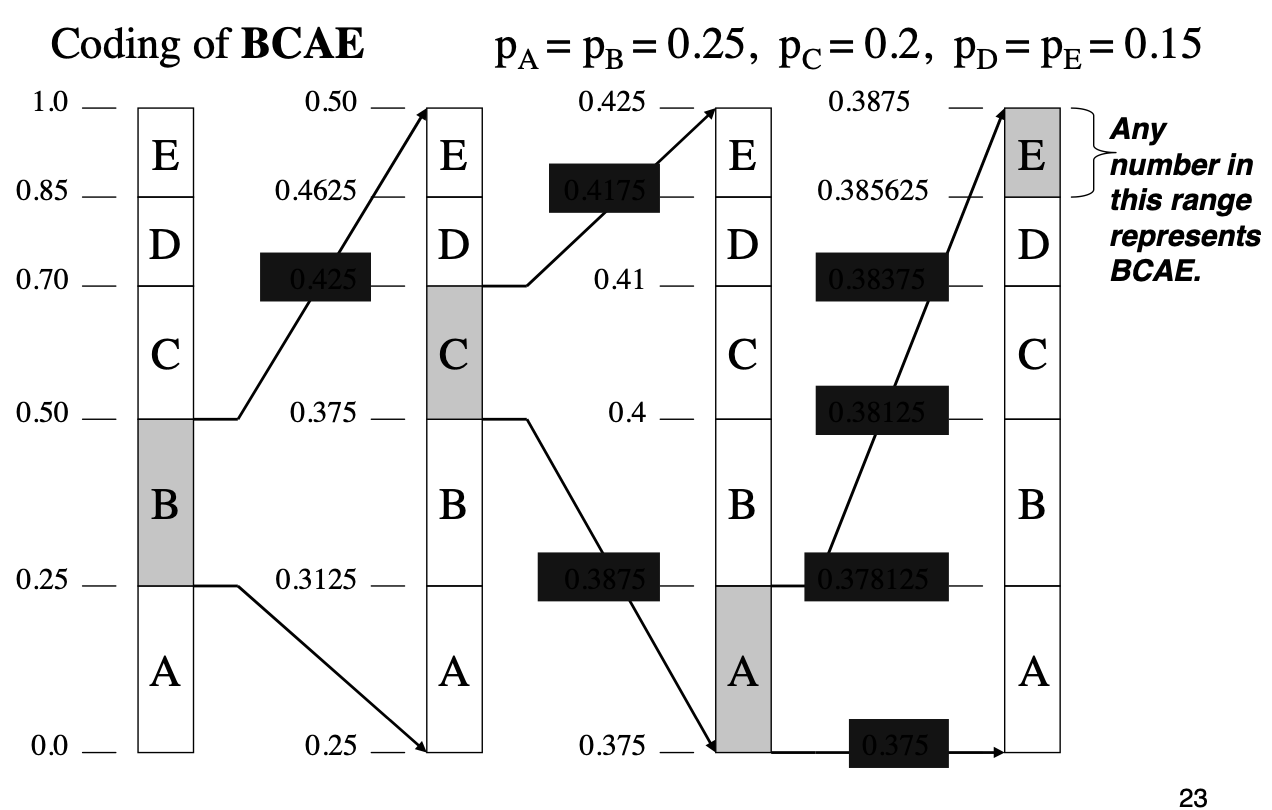
\includegraphics[width=0.6\textwidth]{../24ws_ANS.assets/fig21.png} \\
        source: http://www.math.tau.ac.il/~dcor/Graphics/adv-slides/entropy.pdf
    \end{center}
\end{frame}